\section{Понятие двойного и повторного пределов. Теорема о связи
двойных и повторных пределов}

\subsection{Определение двойного предела (предел функции двух
переменных)}

При рассмотрении предела функции одной переменной \(y=f(x)\) было
введено понятие окрестности точки \(x_{0}\). Для рассмотрения предела
функции двух переменных \(z=f\left(x, y\right)=f(P)\) будем
рассматривать окрестность точки в плоскости \(Oxy\).

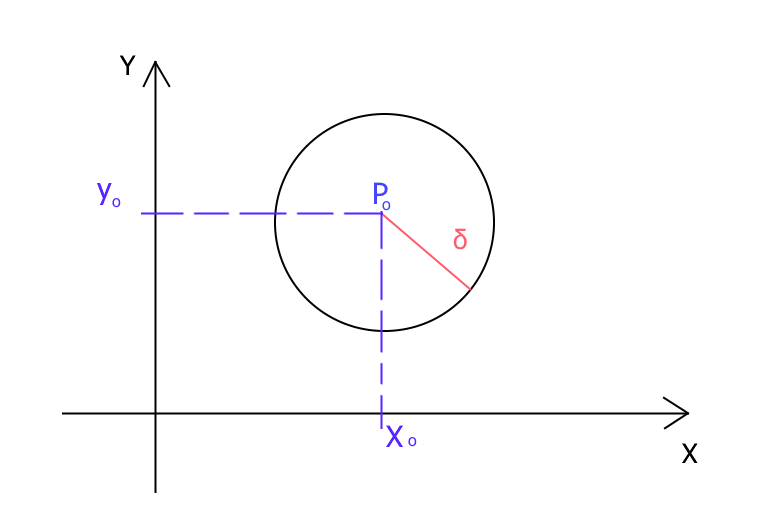
\includegraphics[width=\linewidth]{10img.png}

Окрестностью точки \(P_{0}\left(x_{0}; y_{0}\right)\) называется
внутренность круга с центром в этой точке. Радиус круга равен
\(\delta\). Очевидно, что любая точка \(P\left(x; y\right)\) \(\delta\)
- окрестности точки \(P_{0}\left(x_{0}; y_{0}\right)\) находится от этой
точки на расстоянии, меньшем \(\delta\).

\subsubsection{Определение.}

Число \(b\) называют пределом функции \(z=f(x, y)=f(P)\) при
\(P \rightarrow P_{0}\), если для
\(\forall \varepsilon>0 \quad \exists \delta\) - окрестность точки
\(P_{0}\left(x_{0}; y_{0}\right)\) , что для \(\forall\)
\(P\left(x; y\right)\) точки этой окресности, имеет место равенство:

\[
|f(P)-b|
<\varepsilon
\]

или \[
|f(x, y)-b|
<\varepsilon
\]

При этом пишут \(\lim _{P \rightarrow P_{0}} f(P)=b \quad\) или
\(\ \ \lim _{x \rightarrow x_{0} \atop y \rightarrow y_{0}} f(x, y)=b,\)
так как при \(P(x ; y) \rightarrow P_{0}\left(x_{0} ; y_{0}\right),\)
следует, \(x \rightarrow x_{0}, y \rightarrow y_{0}\) (в силу критерия
сходимости в пространстве \(\mathbb{R}^{n}\) )

\subsection{Повторный предел}

\subsubsection{Определение}

Для функции \(u=f\left(x_{1}, x_{2}, \ldots, x_{m}\right)\) нескольких
переменных можно определить понятие предела по одной из переменных
\(x_{k}\) при фиксированных значениях остальных переменных. В связи с
этим возникает понятие повторного предела. Уясним это понятие на примере
функции \(u=f(x, y)\). Пусть функция \(u=f(x, y)\) задана в некоторой
прямоугольной окрестности
\(0<\left|x-x_{0}\right|<d_{1},0<\left|y-y_{0}\right|<d_{2}\) точки
\(M_{0}\left(x_{0}, y_{0}\right)\), за исключением, быть может, самой
точки \(M_{0}\). Пусть для каждого фиксированного ``y'',
удовлетворяющего условию \(0<\left|y-y_{0}\right|<d_{2}\), существует
предел функции \(u=f(x, y)\) одной переменной \(x\) в точке \(x=x_{0}\):

\[\lim _{x \rightarrow x_{0} \atop y-\text {фикс }} f(x, y)=\varphi(y)\]

и пусть, кроме того, существует предел \(b\) функции \(\varphi(y)\) в
точке \(y=y_{0}\):

\[\lim _{y \rightarrow y_{0}} \varphi(y)=b\]

В этом случае говорят, что существует повторный предел \(b\) для функции
\(u=f(x, y)\) в точке \(M_{0}\), который обозначается следующим образом:

\[\lim _{y \rightarrow y_{0}} \lim _{x \rightarrow x_{0}} f(x, y)=b\]

Аналогично определяется повторный предел:

\[\lim _{x \rightarrow x_{0}} \lim _{y \rightarrow y_{0}} f(x, y)\]

\subsection{Теорема о связи двойных и повторных пределов}

Обратимся к вышеописанной функции \(u=f(x, y)\). Если:

\[\exists\lim _{x \rightarrow x_{0} \atop y \rightarrow y_{0} } f(x, y)=A\]

Пусть \(\forall\)\(x\): \(0<\left|x-x_{0}\right|<\delta_{1}\):
\[\exists\lim _{y \rightarrow y_{0}} f(x, y)=\varphi(x)\]

Тогда:

\[\exists\lim _{x \rightarrow x_{0}} \varphi(x)=A\]

Что равносильно:

\[\lim _{x \rightarrow x_{0}} \lim _{y \rightarrow y_{0}} f(x, y)=\lim _{x \rightarrow x_{0} \atop y \rightarrow y_{0}} f(x, y)=A\]

\subsubsection{Доказательство}

\(\forall \epsilon\)\textgreater{}0 \(\exists\)
\(\delta_{1}(\epsilon) > 0:\)
\(\forall M(x,y):\)\(0<\rho\)(\(M_{1}\),\(M_{0}\))\textless{}\(\delta_{1}\)
\(\Rightarrow\) \(\left|f(x,y)-A\right|<\epsilon/ 2\)

где: \(\rho\)(\(M_{1}\),\(M_{0}\)) = \(\max(|x-x_{0}|,| y-y_{0}|)\)
\(<\) \(\delta_{1}\)

\(\forall x:0<|x-x_{0}|<\delta:\)
\(\ \ \forall \epsilon\)\textgreater{}0\(:\)
\(\exists \delta_{2}(\epsilon,x)>0:\) \(\forall y:\)
\(0<\left|y-y_{0}\right|<\delta_{2}\) \(\Rightarrow\)
\(\left|f(x,y)-\varphi(x)\right|<\epsilon/ 2\)

\(\left|\varphi(x)-A\right|\leq\)
\(|f(x, y)-\varphi(x)|+| f(x, y)-A|\)\(<\) \(|f(x, y)-\varphi(x)|\) +
\(\epsilon/2<\) \(\epsilon/ 2<\) + \(\epsilon/ 2\)=\(\epsilon\)

Ход преобразований: \\
1) Отнимем и прибавим функцию \(f(x,y)\) \\
2)\(| f(x, y)-A|\) \(< \epsilon /2\), если: \(\max(|x-x_{0}|,| y-y_{0}|)\) \\
\(<\) \(\delta_{1}\), следовательно сделаем условие для преобразования: \\

\[\left\{\begin{array}{l}
0<\left|x-x_{0}\right|<\delta_{1} \\
0<\left|y-y_{0}\right|<\delta_{1}
\end{array}\right.\]

\begin{enumerate}
\def\labelenumi{\arabic{enumi})}
\setcounter{enumi}{2}
\tightlist
\item
  \(|f(x, y)-\varphi(x)|\) \textless{} \(\epsilon /2\), если: \(x:\)
  \(0<\left|x-x_{0}\right|<\delta_{1}:\)
  \(\exists \delta_{2}(\epsilon, x)\), также условие для \textbf{y}:
\end{enumerate}

\[\left\{\begin{array}{l}
0<\left|y-y_{0}\right|<\delta_{2}(\epsilon, x) \\
0<\left|y-y_{0}\right|<\delta_{1}(\epsilon)
\end{array}\right.\]
